\documentclass[preprint]{elsarticle}
\usepackage[margin=1in, bottom=1in, top=1in]{geometry} %1 inch margins
\usepackage{amsmath, amssymb, amstext}
\usepackage{fancyhdr}
\usepackage{algorithm}
\usepackage{algpseudocode}
\usepackage{mathtools}
\usepackage{theorem}
\usepackage{xcolor}
\usepackage{tikz}
\usetikzlibrary[topaths]
\usetikzlibrary{decorations.pathmorphing}
\DeclarePairedDelimiter{\ceil}{\lceil}{\rceil}
\DeclarePairedDelimiter\floor{\lfloor}{\rfloor}

%Theorem
\newtheorem{fact}{Fact}[section]
\newtheorem{lemma}[fact]{Lemma}
\newtheorem{theorem}[fact]{Theorem}
\newtheorem{definition}[fact]{Definition}
\newtheorem{corollary}[fact]{Corollary}
\newtheorem{proposition}[fact]{Proposition}
\newtheorem{claim}[fact]{Claim}
\newtheorem{exercise}[fact]{Exercise}
\newtheorem{note}[fact]{Note}
\newenvironment{proof}{{\bf Proof:  }}{\hfill\rule{2mm}{2mm}}
%Macros
\newcommand{\A}{\mathbb{A}} \newcommand{\C}{\mathbb{C}}
\newcommand{\D}{\mathbb{D}} \newcommand{\F}{\mathbb{F}}
\newcommand{\N}{\mathbb{N}} \newcommand{\R}{\mathbb{R}}
\newcommand{\T}{\mathbb{T}} \newcommand{\Z}{\mathbb{Z}}
\newcommand{\Q}{\mathbb{Q}}
 
 
\newcommand{\cA}{\mathcal{A}} \newcommand{\cB}{\mathcal{B}}
\newcommand{\cC}{\mathcal{C}} \newcommand{\cD}{\mathcal{D}}
\newcommand{\cE}{\mathcal{E}} \newcommand{\cF}{\mathcal{F}}
\newcommand{\cG}{\mathcal{G}} \newcommand{\cH}{\mathcal{H}}
\newcommand{\cI}{\mathcal{I}} \newcommand{\cJ}{\mathcal{J}}
\newcommand{\cK}{\mathcal{K}} \newcommand{\cL}{\mathcal{L}}
\newcommand{\cM}{\mathcal{M}} \newcommand{\cN}{\mathcal{N}}
\newcommand{\cO}{\mathcal{O}} \newcommand{\cP}{\mathcal{P}}
\newcommand{\cQ}{\mathcal{Q}} \newcommand{\cR}{\mathcal{R}}
\newcommand{\cS}{\mathcal{S}} \newcommand{\cT}{\mathcal{T}}
\newcommand{\cU}{\mathcal{U}} \newcommand{\cV}{\mathcal{V}}
\newcommand{\cW}{\mathcal{W}} \newcommand{\cX}{\mathcal{X}}
\newcommand{\cY}{\mathcal{Y}} \newcommand{\cZ}{\mathcal{Z}}


\DeclareMathOperator{\convOp}{conv}
\newcommand{\conv}{\convOp}


\begin{document}
\begin{frontmatter}
%% Title, authors and addresses

%% use the tnoteref command within \title for footnotes;
%% use the tnotetext command for the associated footnote;
%% use the fnref command within \author or \address for footnotes;
%% use the fntext command for the associated footnote;
%% use the corref command within \author for corresponding author footnotes;
%% use the cortext command for the associated footnote;
%% use the ead command for the email address,
%% and the form \ead[url] for the home page:
%%
%% \title{Title\tnoteref{label1}}
%% \tnotetext[label1]{}
%% \author{Name\corref{cor1}\fnref{label2}}
%% \ead{email address}
%% \ead[url]{home page}
%% \fntext[label2]{}
%% \cortext[cor1]{}
%% \address{Address\fnref{label3}}
%% \fntext[label3]{}

%% use optional labels to link authors explicitly to addresses:
%% \author[label1,label2]{<author name>}
%% \address[label1]{<address>}
%% \address[label2]{<address>}

\title{The Power of Locality: An Elementary Integrality
  Proof of Rothblum's Stable Matching Formulation}
\author[co]{Jochen K\"{o}nemann}
\author[co]{Kanstantsin Pashkovich}
\author[co]{Justin Toth\corref{cor1}}
\ead{wjtoth@uwaterloo.ca}
\address[co]{Department of Combinatorics and Optimization, University of Waterloo, Canada}

\cortext[cor1]{Corresponding author}

\begin{abstract}
  In this paper we consider Rothblum's linear description of the
  convex hull of incidence vectors of stable matchings in bipartite
  graphs. We provide a short and surprisingly elementary proof that
  leverages only the existence of a local $0,1$-edge to achieve global
  integrality.
\end{abstract}
\begin{keyword}
Stable Matching\sep Polytope\sep Extreme Points
\end{keyword}
\end{frontmatter}
{\color{red}
\section*{TODO}
\begin{enumerate}
	\item citation for structure of symmetric difference, adjacencies in the stable matching polytope
	\item expand some explanations or make them clearer, if necessary: do Lemma 3.1 and Cor 3.2 have sufficient detail?
\end{enumerate}
}

\section{Introduction}

In an instance of the {\em stable marriage} problem, we are given a
bipartite graph $G=(\cA \cup \cB, E)$ where $\cA$ and $\cB$
traditionally represent sets of women and men, respectively. An edge
$ab \in E$ corresponds to an {\em acceptable} pair $a$ and $b$ of man
and woman. In the following, we let $N(u) = \{ v \,:\, uv \in E \}$ be
the set of neighbours of $u$ in $G$. Each vertex
$u \in V=\cA \cup \cB$ specifies a complete {\em preference order}
$>_u$ over its neighbours where vertex $u$ prefers neighbour $v_1$
over $v_2$ iff $v_1 >_u v_2$.  In their seminal paper
\cite{gale1962college}, Gale and Shapley introduced the above problem,
and provided a constructive proof of existence of so called {\em
  stable} matchings. A matching is a collection $M$ of edges in $E$
such that each vertex is incident to at most one edge in $M$. $M$ is
stable if, for all $uv \not\in M$, $M(u) >_u v$ or $M(v) >_v u$ where
$M(u)$ is the vertex matched to $u$ in $M$ if that exists, and
$M(u)=\varnothing$, otherwise.

In this paper, we focus on polyhedral characterizations of the set of
incidence vectors of stable matchings.  Vande Vate first provided such
a description in \cite{vate1989linear} for the special case where $G$
is a complete bipartite graph.  Rothblum
\cite{rothblum1992characterization} later generalized Vande Vate's
result to incomplete preference lists and simplified the proof of
integrality.

We provide an even simpler, more compact argument for the integrality
of Rothblum's formulation. Our proof is inspired by the technique of
{\em iterative rounding} as outlined in Lau et al.'s
monograph~\cite{lau2011iterative}. Our arguments are elementary and
rely solely on some well-known results on the symmetric difference
of stable matchings as well as some knowledge of the local structure
of a variable in our formulation to achieve the desired result.

\section{Stable matchings: Preliminaries}

We briefly review a couple of well-known facts on stable matchings. 
For each edge $uv$ in $E$, we let
$\delta^{>u}(v):=\{ \{v,w\}\in E: w >_v u \}$ to be the set of edges
incident to $v$ those of its neighbours that are preferred to $u$. 
For $v \in V$ let $N_{\max}(v)$ denote its highest-ranked neighbour. 
For ease of notation, we will from now on think of $>_v$ as a total
ordering on $N(v) \cup \varnothing$ where 
$\varnothing$ is the lowest-ranked element of each vertex $v \in V$. 
A matching $M$ in $G$ is now easily seen to be stable if 
\begin{equation}\label{eq:stability_def}
		M \, \cap \, \big(\delta^{>u}(v) \cup \delta^{>v}(u) \cup  \{e\} \big)\neq\varnothing\,,
\end{equation}
for all $uv \in E$. The following lemmas study the connected components of
the {\em symmetric difference} $M_1\triangle M_2:=M_1\setminus M_2
\cup M_2 \setminus M_1$ of 
stable matchings $M_1$ and $M_2$. Here, $V(C)$ and $E(C)$ denote
the set of vertices and edges, respectively, of a graph $C$.

\begin{lemma}\label{lemma:pref}
Let $M_1$ and $M_2$ be two stable matchings in $G$ and let $C$ be a
connected component in $M_1 \triangle M_2$. Then for some
$\{i,j\}=\{1,2\}$, we have
\begin{equation}\label{eq:pref}
	M_i(a)>_a M_j(a) ~~\text{and} ~~  M_j(b)>_b M_i(b)\,,\,
\end{equation}
for all $a \in V(C) \cap \cA$ and $v \in V(C) \cap \cB$.
\end{lemma}
\begin{proof}
  Since $M_1$ and $M_2$ are matchings, $C$ is a path or a cycle. Let
  $v\in V$ be an end node of $C$ if $C$ is a path, otherwise let $v$
  be an arbitrary node of $C$.

  W.l.o.g. $v:=a\in \mathcal{A}$ and $b:=M_1(a) >_a M_2(a)$. If
  $a=M_1(b) >_b M_2(b)$, the matching $M_2$
  violates~\eqref{eq:stability_def} for the edge $ab\in E$. Thus,
  $M_2(b) >_b M_1(b)=a$. Thus, $M_2(b)\neq \varnothing$ and the
  matching $M_1$ satisfies~\eqref{eq:stability_def} for the edge
  $e:=bM_2(b)\in E$ only if $M_1(M_2(b))>_{M_2(b)} b$. Continuing
  in this way, we obtain statement~\eqref{eq:pref}.
\end{proof}

\begin{figure}[H]
\centering
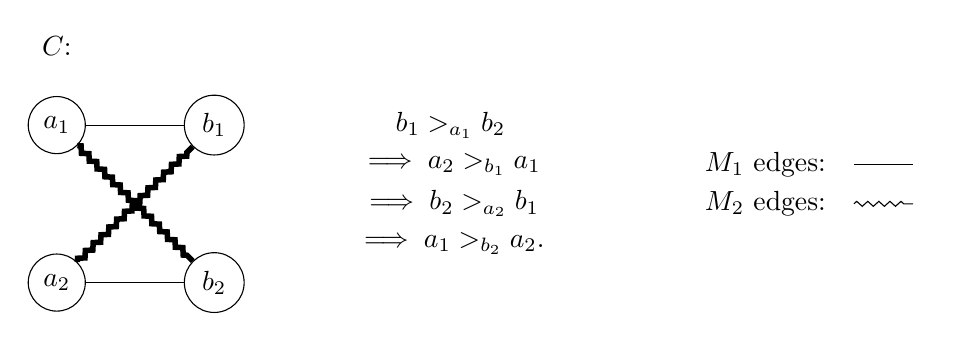
\begin{tikzpicture}
\node[] (J1) at (0,5) {$C$:};

\node[shape=circle,draw=black] (1) at (0,4) {$a_1$};
\node[shape=circle,draw=black](2) at (2,4){$b_1$};
\node[shape=circle,draw=black] (3) at (0,2) {$a_2$};
\node[shape=circle,draw=black](4) at (2,2){$b_2$};

\path[-] (1) edge  (2);
\path[-,line width=2pt,decoration={zigzag,segment length=4,amplitude=.9,post=lineto,post length=2pt}] (1) edge[decorate] (4);
\path[-] (3) edge (4);
\path[-,line width=2pt,decoration={zigzag,segment length=4,amplitude=.9,post=lineto,post length=2pt}] (3) edge[decorate] (2);

\node[](M1) at (9,3.5) {$M_1$ edges:};
\node[](m11) at (10,3.5){};
\node[](m12) at (11,3.5){};
\path[-](m11) edge(m12);
\node[](M2) at (9,3) {$M_2$ edges:};
\node[](m21) at (10,3){};
\node[](m22) at (11,3){};
\path[-,decoration={zigzag,segment length=4,amplitude=.9,post=lineto,post length=2pt}](m21) edge[decorate](m22);

\node[](a) at (5, 4) {$b_1 >_{a_1} b_2$};
\node[](b) at (5,3.5) {$\implies a_ 2 >_{b_1} a_1$};
\node[](c) at (5,3) {$\implies b_2 >_{a_2} b_1$};
\node[](d) at (5,2.5) {$\implies a_1 >_{b_2} a_2.$};

\end{tikzpicture}
\caption{Visualizing Lemma \ref{lemma:pref}. If any implication above doesn't hold, a blocking pair is found for the other matching.}
\end{figure}

\begin{lemma}\label{lemma:sym_stable} 
  Let $M_1$ and $M_2$ be two stable matchings in $G$. Let $J_1$ be
  those connected components of $M_1 \triangle M_2$ 
  that satisfy
  \eqref{eq:pref} for $i=1$ and $j=2$ (i.e., $\cA$ vertices prefer
  $M_1$ edges); let $J_2$ be all
  remaining connected components of $M_1 \triangle M_2$. 
  Then both $M'_1 = M_1\triangle J_1$ and
  $M'_2=M_1\triangle J_2$ are stable matchings in $G$.
\end{lemma}
\begin{proof}
  For contradiction assume
  that one of the matchings $M'_1$ and $M'_2$ is not stable; w.l.o.g. assume that
  $M'_1$ does not satisfy~\eqref{eq:stability_def} for some edge
  $ab\in E$ with $a\in\mathcal{A}$ and $b\in\mathcal{B}$.

  Since $M_1$ and $M_2$ are stable, $a$ and $b$ cannot both lie in the
  same connected component of $J_1 \cup J_2$. Suppose first that $a \in
  V(J_1)$, and $b \in V(J_2)$. In this case $M'_1(a)=M_2(a)$ and
  $M'_1(b) = M_1(b) >_b M_2(b)$. Thus $M_2$
  violates~\eqref{eq:stability_def} for edge $ab$. 

  If $a\in V(J_2)$
  and $b\in V(J_1)$, then $M'_1(a)=M_1(a)$ and $M'_1(b)>_b M_1(b)$,
  and hence $M_1$ violates~\eqref{eq:stability_def} for edge $ab$,
  contradiction.
\end{proof}

\begin{figure}[H]
\centering
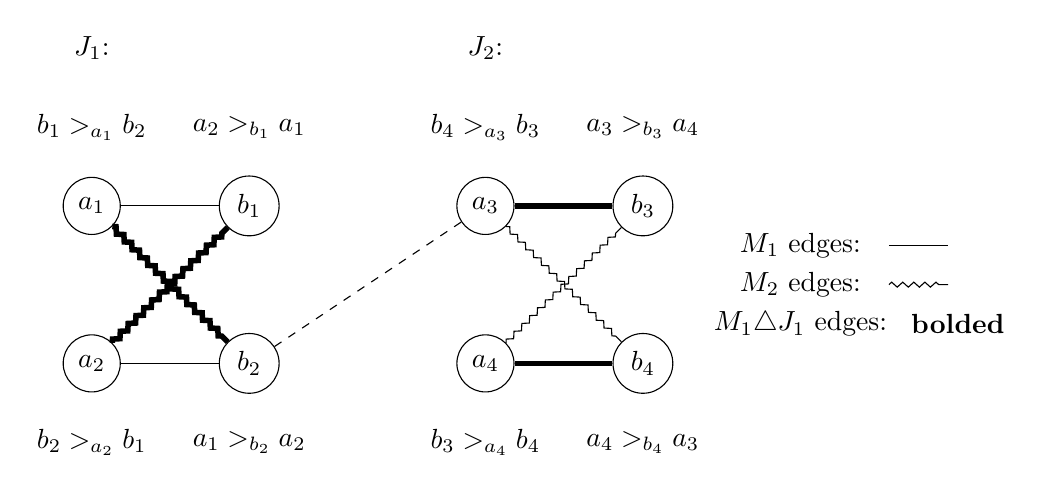
\begin{tikzpicture}
\node[] (J1) at (0,6) {$J_1$:};

\node[shape=circle,draw=black] (1) at (0,4) {$a_1$};
\node[shape=circle,draw=black](2) at (2,4){$b_1$};
\node[shape=circle,draw=black] (3) at (0,2) {$a_2$};
\node[shape=circle,draw=black](4) at (2,2){$b_2$};

\path[-] (1) edge  (2);
\path[-,line width=2pt,decoration={zigzag,segment length=4,amplitude=.9,post=lineto,post length=2pt}] (1) edge[decorate] (4);
\path[-] (3) edge (4);
\path[-,line width=2pt,decoration={zigzag,segment length=4,amplitude=.9,post=lineto,post length=2pt}] (3) edge[decorate] (2);

\node[] (J2) at (5,6) {$J_2$:};

\node[shape=circle,draw=black] (5) at (5,4) {$a_3$};
\node[shape=circle,draw=black](6) at (7,4){$b_3$};
\node[shape=circle,draw=black] (7) at (5,2) {$a_4$};
\node[shape=circle,draw=black](8) at (7,2){$b_4$};

\path[-,line width=2pt] (5) edge  (6);
\path[-,decoration={zigzag,segment length=4,amplitude=.9,post=lineto,post length=2pt}] (5) edge[decorate] (8);
\path[-,line width=2pt] (7) edge (8);
\path[-,decoration={zigzag,segment length=4,amplitude=.9,post=lineto,post length=2pt}] (7) edge[decorate] (6);

\node[](M1) at (9,3.5) {$M_1$ edges:};
\node[](m11) at (10,3.5){};
\node[](m12) at (11,3.5){};
\path[-](m11) edge(m12);
\node[](M2) at (9,3) {$M_2$ edges:};
\node[](m21) at (10,3){};
\node[](m22) at (11,3){};
\path[-,decoration={zigzag,segment length=4,amplitude=.9,post=lineto,post length=2pt}](m21) edge[decorate](m22);
\node[](m1j1) at (9,2.5){$M_1\triangle J_1$ edges:};
\node[](bolded) at (11,2.5){$\textbf{bolded}$};

\node[]() at (0, 5) {$b_1 >_{a_1} b_2$};
\node[]() at (2, 5) {$a_2 >_{b_1} a_1$};
\node[]() at (0, 1) {$b_2 >_{a_2} b_1$};
\node[]() at (2,1) {$a_1 >_{b_2} a_2$};

\node[]() at (5, 5) {$b_4 >_{a_3} b_3$};
\node[]() at (7, 5) {$a_3 >_{b_3} a_4$};
\node[]() at (5, 1) {$b_3 >_{a_4} b_4$};
\node[]() at (7,1) {$a_4 >_{b_4} a_3$};

\path[dashed](4) edge (5);
\end{tikzpicture}
\caption{Visualizing Lemma \ref{lemma:sym_stable}. If $b_2a_3$ blocks $M_1 \triangle J_1$ then $b_2a_3$ blocks $M_1$.}
\end{figure}

\section{Stable Matching Polytope}

Let us define the \emph{stable matching polytope} $P(G)\subseteq\R^E$ for graph $G$ as follows
$$
	P(G):=\conv\{\chi(M)\in\R^E: M \text{ is a stable matching in } G\}\,.
$$
By~\cite{gale1962college}, $P(G)$ is a nonempty polytope because every
graph $G$ has a stable matching.

Clearly, the vertices of $P(G)$ are in one-to-one correspondence with
stable matchings in $G$. Moreover, Lemma~\ref{lemma:sym_stable} helps
to understand what pairs of stable matchings in $G$ do not correspond
to edges of $P(G)$.

\begin{lemma}\label{lemma:edge}
  Let $M_1$ and $M_2$ be two stable matchings in $G$ which define an
  edge of the polytope~$P(G)$. 
  Then all connected components in
  $M_1\triangle M_2$ satisfy~\eqref{eq:pref} for unique choice of $i$
  and $j$. 
\end{lemma}
\begin{proof}
  Suppose for contradiction that the statement of the lemma does not
  hold. Hence the sets $J_1$ and $J_2$ are both nonempty in
  Lemma~\ref{lemma:sym_stable}, and we obtain stable matchings
  $M_1\triangle J_1$ and $M_1\triangle J_2$ that are different from $M_1$,
  $M_2$. 
  We also have 
  \[ \frac{1}{2}\chi(M_1\triangle J_1)+\frac{1}{2}\chi(M_1\triangle
  J_2) =\frac{1}{2}\chi(M_1)+\frac{1}{2}\chi(M_2),\]
  and hence there are two distinct convex combinations of the midpoint
  of the edge between $M_1$ and $M_2$; a contradiction. 
\end{proof}


\begin{corollary}\label{cor:edge}
Let $M_1$ and $M_2$ be two stable matchings in $G$ such that
\begin{equation}\label{eq:edge}
M_1\cap\delta^{>a}(b)\neq\varnothing,\
M_1\cap\delta^{>b}(a)\neq\varnothing\quad\text{and}\quad
M_2\cap\big(\delta^{>a}(b)\cup \delta^{>b}(a)\big)=\varnothing
\end{equation}
 for some $a\in\mathcal{A}$ and $b\in\mathcal{B}$. Then, $M_1$ and $M_2$ do not define an edge of the polytope~$P(G)$.
\end{corollary}
\begin{proof}
  Condition \eqref{eq:edge} implies that both $a$ and $b$ prefer
  $M_1$ over $M_2$. Hence, both sets $J_1$ and $J_2$ as given in Lemma
  \ref{lemma:sym_stable} must be non-empty. An application of Lemma
  \ref{lemma:edge} completes the proof of the corollary.
\end{proof}


\section{Linear Description}
Let us define $Q(G)\subseteq\R^E$ to be the polytope described by the
following linear constraints
\begin{align}
  x(\delta(v)) \leq 1\,,\quad \forall v \in V\qquad \text{and} \qquad x_e \geq 0\,,\quad \forall e \in E\,,\label{eq:lin_descr_match}\\
  x(\delta^{>a}(b))+ x(\delta^{>b}(a)) + x_{ab} \geq 1\,, \quad \forall ab \in E \label{eq:lin_descr_stab}
\end{align}
where $x(J) = \sum_{e \in J} x_e$ for any $J \subseteq E$.

Clearly, $P(G)\subseteq Q(G)$ because for every stable matching $M$ in
$G$ the point $x:=\chi(M)$ satisfies~\eqref{eq:lin_descr_match} and
by~\eqref{eq:stability_def} the point $x$ also
satisfies~\eqref{eq:lin_descr_stab}. On the other hand, every integral
point in $Q(G)$ equals $\chi(M)$ for some stable matching $M$
in~$G$. In the remaining part of the paper we show that every vertex
of $Q(G)$ is integral, thus proving the main theorem.

\begin{theorem}
	For every graph $G$ the polytope $P(G)$ equals $Q(G)$.
\end{theorem}


\begin{lemma}
	For every graph $G$ every vertex of the polytope $Q(G)$ is integral.
\end{lemma}
\begin{proof}
  We first claim that every vertex $x$ of $Q(G)$ satisfies $x_e
  \in \{0,1\}$ for at least one $e \in E$. Assume for contradiction
  that $0 < x_e < 1$ for all $e \in E$. Hence, $x$ is uniquely defined 
  by $|E|$ linearly independent tight constraints
  describing $Q(G)$. Since $x$ has no zero coordinate, we can assume
  that the tight constraints are $x(\delta(v))\le 1$ for $v\in V_x$
  and \eqref{eq:lin_descr_stab} for $e\in E_x$, where
  $|V_x|+|E_x|=|E|$. Moreover, let us assume that we choose the $|E|$
  tight constraints so that $|V_x|$ is as large as possible.

The constraints $x(\delta(v))=1$, $v\in V$ are linearly dependent, in particular $\sum_{a\in\mathcal{A}}\chi(\delta(a))=\sum_{b\in\mathcal{B}}\chi(\delta(b))$. Hence, we have $V_x\subsetneq V$. On the other hand if $a=N_{\max}(b)$ then $e:=ab\not\in E_x$. Indeed, $a=N_{\max}(b)$ implies $\delta^{>a}(b)=\varnothing$ then
$$
	1\le x(\delta^{>a}(b))+ x(\delta^{>b}(a)) + x_{ab}=x(\delta^{\ge b}(a)) \le x(\delta(a)) \le 1\,,
$$
showing that $\delta^{< b}(a)=\varnothing$ and hence $E_x\setminus e$, $V_x\cup \{a\}$ also define the vertex $x$. Analogously, we can show that if $b\in V_x$  and $a=N_{\min}(b)$ then $e:=ab\not\in E_x$. Moreover, notice that $N_{\min}(v)\neq N_{\max}(v)$ for $v\in V_x$ since no coordinate of $x$ equals $1$. Thus, 
\[
	|E_x|=\frac{1}{2}\sum_{v\in V} |\delta(v)\cap E_x|\le \frac{1}{2}\sum_{v\in V_x} (|\delta(v)|-2)+\frac{1}{2}\sum_{v\in V\setminus V_x} (|\delta(v)|-1)= |E|-|V_x|-\frac{1}{2}|V\setminus V_x|\,,
\]
which implies $|E_x|+|V_x|< |E|$, contradiction.

\bigskip

Now let us assume that $G$ is a graph with the minimum number of edges such that $Q(G)$ is not an integral polytope. Let $x$ be a non-integral vertex of $Q(G)$.

Case $x_{ab}=0$ for some $a\in \mathcal{A}$, $b\in\mathcal{B}$ and
$e:=ab\in E$. In this case, let $x'$ be obtained from $x$ by dropping
the coordinate corresponding to $ab$, and let $G'$ be the graph with
$V(G')=V$ and $E(G') = E \setminus \{e\}$. Define $H'$ to be the
hyperplane
$\{x\in \R^{E(G')}: x(\delta^{>a}(b))+ x(\delta^{>b}(a))=1\}$. Then,
$x'$ is a vertex of the polytope $P':=P(G')\cap H'$.  But every vertex
of $P'$ is either a vertex of $P(G')$ or the intersection of an edge
of $P(G')$ with the hyperplane $H'$. Since vertices of $P(G')$ are
integral by the minimal choice of graph $G$, it remains to consider
vertices at the intersection of $H'$ and an edge of $P(G')$. Such an
edge would be defined by stable matchings $M_1$ and $M_2$ that are
easily checked to satisfy \eqref{eq:edge} for the given edge $ab$.
Corollary \ref{cor:edge} therefore readily implies that $P(G')$ cannot
have an edge connecting $M_1$ and $M_2$.

Case $x_{ab}=1$ for some $a\in \mathcal{A}$, $b\in\mathcal{B}$. Let
$x'$ be obtained by dropping the coordinates corresponding to
$\delta(a)\cup\delta(b)$, and let $G'$ be the graph with
$V(G')=V\setminus\{a,b\}$ and
$E(G') = E \setminus \big(\delta(a)\cup\delta(b)\big)$. It is
straightforward to see that $x'$ is a vertex of $P(G')$. Thus by
minimality of $G$ both $x'$ and $x$ are integral, a contradiction.
\end{proof}


\bibliographystyle{alpha}
\bibliography{StableMatchingPolytopeReferences}
\end{document}
